%
%   Dr.HD
%   "robocon.tex"
%

\documentclass[10pt,b5paper,papersize,dvipdfmx]{jsbook}

\usepackage{vuccaken}
\usepackage{vuccaken2019}

% スタイルファイルの読み込みや自作マクロは、
% 最終的には vuccaken2019.sty の中に書いてください。
% とりあえずはここに書いてもらって構いません。


\begin{document} % 以下本文

\setcounter{tocdepth}{2} % 目次にどこまで表示するか
\tableofcontents % 目次出力
\setcounter{page}{0}
\clearpage % 改ページ

% - - - - - - - - - - - - - - - - - - - - - - - - %
\kaishititle%
  {ロボットアーム設計の為の基礎計算}% title
  {ロボティクス学科4回生}% 所属
  {阿部龍幸}% name
% - - - - - - - - - - - - - - - - - - - - - - - - %

\begin{figure}[htbp]
  \centering
  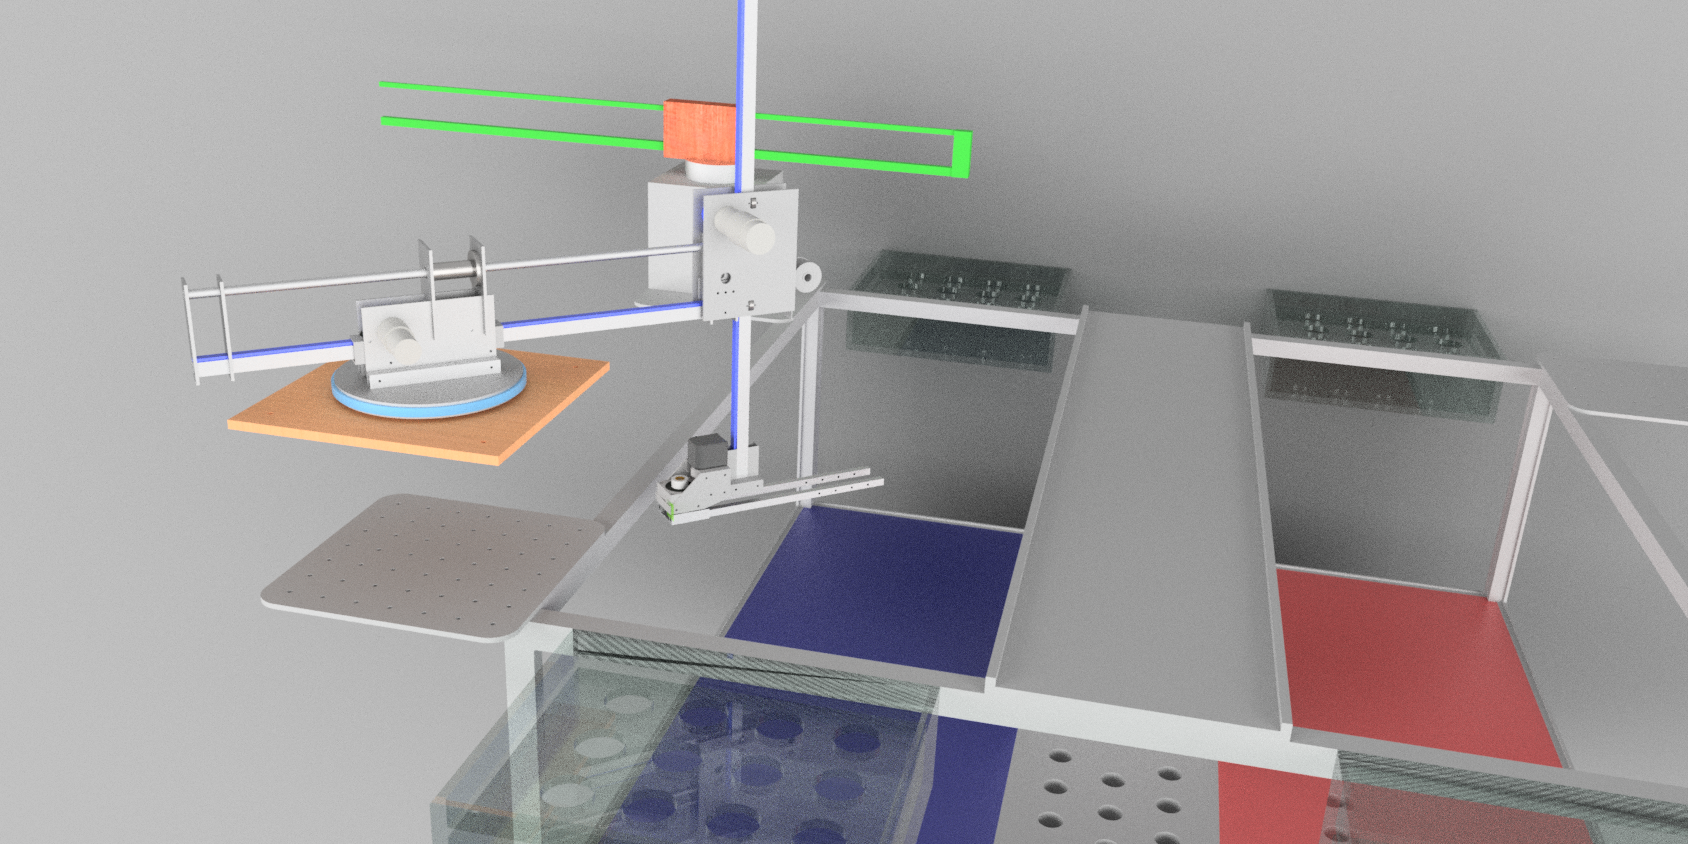
\includegraphics[width=10cm]{robocon/robot_and_field.png}
  % \caption{$y=\sin x$のグラフ。gnuplotで作成した。}
  % \label{fig:robot_and_fields}
\end{figure}

%
\section*{はじめに}
% 会誌ではjsbookクラスを使います。\par
% テーマが複数ある場合は別ファイルで提出してください。
自分が製作予定のロボットアームの最も肝心な一部分の設計をコンピュータによる解析を用いて行う. この設計では, 使用する材質の強度等を考慮しながらアームの形状を変更し, ロボットがユーザの要求する速度を満たすことを目指す. ロボットをCADソフトで設計する際には, 入手可能な材料を以て製作可能な形状を考慮しつつ, 計算に手間のかからない単純な形状を組み合わせたモデルになるように進める. 以下, 物理量をSI単位系で示し, 有効数字を少数点以下2桁とする. 尚, モデルの画像において寸法の表記は[mm]表記とする. 

%
\section{課題設定}
% はじめにこのファイルのソースを自分のtexファイルにコピペしてください。\par
% figureのパスには注意してください。
\subsection{設計目的}
包装されたお菓子などの軽量なワークを素早くハンドリングするロボットアームの, ロボットベースに対して垂直にとった軸周りに素早く回転するアーム部分を設計したい. 回転軸周りのトルク$\tau =1.0 \times 10^3 \tani*{Nm}$ とし, 重力方向の最大変位を $1.0 \times 10^{-2} \tani*{m}$ 以下に抑えることを目指して設計する. また, アームの先には, 実際に製作するロボットが備える機構とハンドを簡略化し, $2.0 \tani*{kg}$ の荷重がかかるパーツを接続する.
\subsection{使用材料}
アームに使用する材料はアルミ合金とする. 主に用いるアルミは6000系で, 押し出し加工性に優れ, 強度が良好で軽量であるという特徴を持つ. これは設計目的にある素早く動くという要求を慣性モーメントの小ささで満たし, 重力方向の最大変位を抑えるという要求を縦弾性係数が満たすと期待できるからである. 他にも板材として2000系アルミ合金を用いるが, 6000系アルミ合金に比べて強度が高く, 使用する部分の殆どが回転軸に近い場所であり慣性抵抗の違いが小さく, また6000系アルミ合金を長手方向に渡って非常に多く使うのでそのひずみの様子重要視したいという理由で今回は全体を6000系アルミとしてモデルを簡単にして計算する. 以降, 密度 $\rho=2.70\times 10^{-6}\tani*{kg/mm^3}$ , 縦弾性係数 $E=68.90 \tani*{GPa}$ , 許容最大応力を $\sigma=2.75×10^{5} \tani*{MPa}$ とする. 安全率はこのアームがロボットの最も基にあり衝撃が加わる可能性がある箇所なので, 余裕を見て $f=15.00$ とする.
\subsection{座標系}
基準座標系をロボットベースの底面とし, リンク座標系を円筒状面の中心に設け, 手先座標系はリンクの先端中央部とし, 解析を行う. 参考となるロボットの構造を図\ref{fig:robot01}に示す. 
\begin{figure}[H]
  \centering
  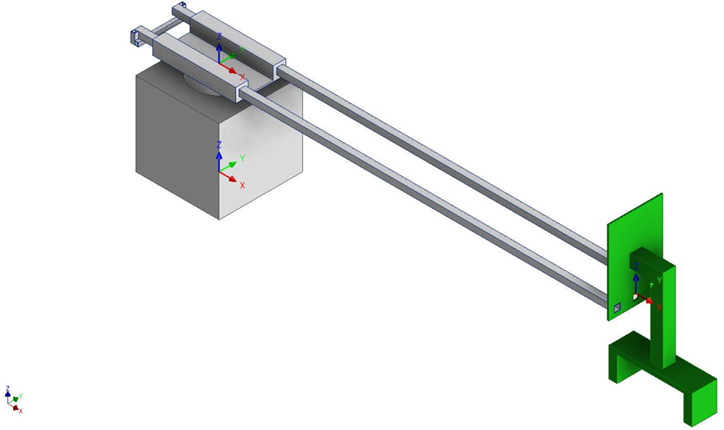
\includegraphics[width=10cm]{robocon/robot01.png}
  \caption{座標系}
  \label{fig:robot01}
\end{figure}
\subsection{基準}
ロボットベースは, 1辺$2.00\times10^{-1} \tani*{m}$ の立方体に直径 $1.20\times10^{-1} \tani*{m} $で,  z 軸方向に上面から $7.00\times10^{-2} \tani*{m}$ の深さの円筒を切り抜いた形状のものとする. 形状を図 2.4.1に示す. 
ロボットアームの, ロボットベースの円筒状の中心から手先までの距離については $1.0\tani*{m}$ に固定とし, ロボットハンドとジョイントの形状はロボットアームに合わせて変更する. また, ジョイントの重量は無視し, ハンドの重量は $2.0\tani*{kg}$ で固定とする. 
ベースとアームを接続するジョイント, ロボットアーム, ロボットハンドの形状については複雑であるので, それぞれFig. 2.4.2, Fig. 2.4.3, Fig. 2.4.4に必要な寸法を示す.

\clearpage
%% 参考文献
\begin{sanko}  \begin{enumerate}
    \item 著者, 本やページの名前, (URL), 出版社, 出版年.
    \item (複数ある場合は追加)
    \item @vuccaken, 物科研HP, \url{rp2017xy.starfree.jp}, 2019.
  \end{enumerate}
\end{sanko}


\end{document}
%
% ファイトだよ!
%
